\documentclass[a4paper,12pt]{report}

\usepackage{../ssumath}

\begin{document}
	
\mktitle{Math 440 -- Real Analysis II}{Exam 2}{Amandeep Gill}

\problem{1}{}{
	\subproof{(a)}{
		The sequence $\{\cos(nx)\}_{n=0}^{\infty}$ is orthogonal on $[-\pi, \pi]$.
	}{
		Let $m,n \in \bb{N} \cup \{0\}$.
		\item[\textbf{case}] $m \not= n$:\\
		\longeq{
			\eqstep{\int_{-\pi}^{\pi}\cos(nx)\cos(mx)dx}{ \int_{-\pi}^{\pi}\frac{1}{2}(\cos(mx - nx) + \cos(mx + nx))dx}
			\eqstep{}{\frac{1}{2}\left(\frac{1}{m-n}sin((m-n)x) + \frac{1}{m+n}sin((m+n)x)\right)_{-\pi}^{\pi}}
			\eqstep{}{0}
		}
		
		\item[\textbf{case}] $m = n \not= 0$:\\
		\longeq{
			\eqstep{\int_{-\pi}^{\pi}\cos(nx)\cos(mx)dx}{\int_{-\pi}^{\pi}\cos^2(mx)dx}
			\eqstep{}{\left(\frac{sin(2mx)}{m} + \pi\right)_{-\pi}^{\pi}}
			\eqstep{}{\pi \not= 0}
		}
		
		\item[\textbf{case}] $m = n = 0$:\\
		Since $\cos(0x) = 1$, $\abrace{1,1} = 2\pi \not= 0$
		
		Therefore the sequence $\{\cos(nx)\}_{n=0}^{\infty}$ is orthogonal on $[-\pi, \pi]$.
	}
	
	\subsoln{(b)}{
		Find the Fourier series of $f(x) = \abs{x}$ on $[-\pi,\pi]$ with respect to the sequence $\{\cos(nx)\}_{n=0}^{\infty}$.
	}{
		$f(x) \sim \sum\limits_{n=0}^{\infty}c_n\cos(nx)$\\
		$\naught{c} = \frac{1}{2\pi}\int_{-\pi}^{\pi}f(x)dx = \frac{\pi}{2}$\\
		$c_n = \frac{1}{\pi}\int_{-\pi}^{\pi}f(x)\cos(nx)dx = \frac{2}{\pi n^2}(\pi n \sin(\pi n) + \cos(\pi n) - 1)$\\
		\piecewise{c_n}{
			\pwcond{0}{n = \text{even}}
			\pwcond{-\frac{4}{\pi n^2}}{n = \text{odd}}
		}
		
		Therefore:\\
		\longeq{
			\eqstep{\sum\limits_{n=0}^{\infty}c_n\cos(nx)}{\frac{\pi}{2} - \frac{4}{\pi}\cos(x) - \frac{4}{9\pi}\cos(3x) - \frac{4}{25\pi}\cos(5x) - \cdots}
			\eqstep{}{\frac{\pi}{2} - \frac{4}{\pi}\left[\cos(x) + \frac{1}{9}\cos(3x) + \frac{1}{25}\cos(5x) + \cdots\right]}
			\eqstep{}{\frac{\pi}{2} - \frac{4}{\pi}\sum\limits_{n=0}^{\infty}\frac{1}{(2n+1)^2}\cos((2n+1)x)}
		}
	}
}

\problem{1}{
	continued...
}{
	\item[\textbf{(c)}]
		Graph the first four $n^\text{th}$ partial sums from (b) with $f(x)$.\\
		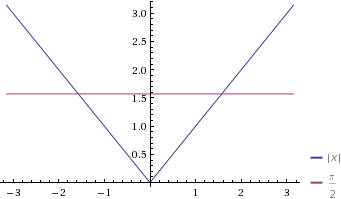
\includegraphics{s0}
		
		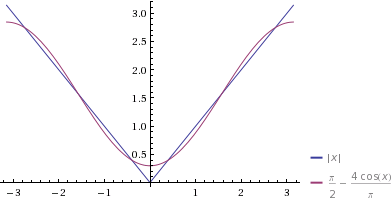
\includegraphics{s1}
		
		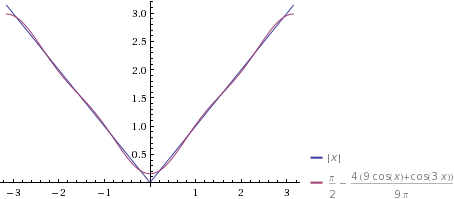
\includegraphics{s3}
		
		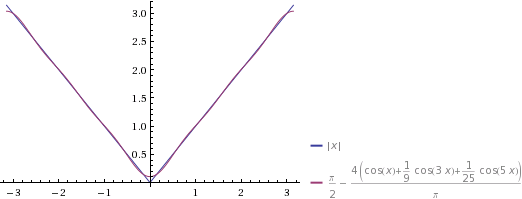
\includegraphics{s5}
}

\pagebreak

\problem{2}{
	Let $K \not= \emptyset$, and $\mathcal{F} = \{f : K \rightarrow \bb{R} : \exists M $ such that $\abs{f(x)} \leqslant M, \forall x \in K\}$. For each $f \in \mathcal{F}$, define $\norm{f} = \sup\limits_{x \in K}\abs{f(x)}$.
}{
	\subproof{(a)}{
		$\mathcal{F}$ is a vector space.
	}{
		Let $f,g \in \mathcal{F}$ such that $\abs{f(x)} \leqslant M_1$ and $\abs{g(x)} \leqslant M_2$ for all $x \in K$. Then $\abs{f(x) + g(x)} \leqslant \abs{f(x)} + \abs{g(x)} \leqslant M_1 + M_2$ for al $x \in K$, thus $(f+g) \in \mathcal{F}$ and $\mathcal{F}$ is closed under vector addition.
		
		Let $f \in \mathcal{F}$ such that $\abs{f(x)} \leqslant M$ and $c \in \bb{R}$. From this, we have $\abs{c \cdot f(x)} = \abs{c} \cdot \abs{f(x)} \leqslant \abs{c} \cdot M$ for all $x \in K$, which means that $c \cdot f \in \mathcal{F}$ for all $c \in \bb{R}$ and $\mathcal{F}$ is closed under scalar multiplication.
		
		Since the eight vector space axioms are assumed trivially, $\mathcal{F}$ is a vector space.
	}
	
	\subproof{(b)}{
		$\left(\mathcal{F},\norm{\cdot}\right)$ is a normed vector space.
	}{
		Let $f,g \in \mathcal{F}$ and $c \in \bb{R}$
		\begin{enumerate}
		\item[(a)] 
			$\norm{f} \geqslant 0$ since for all $x \in K$, $\abs{f(x)} \geqslant 0$, and thus $\sup\limits_{x \in K}\abs{f(x)} \geqslant 0$
		\item[(b)]
			$f(x) = 0$ for all $x \in K$ implies that $\sup\limits_{x \in K}\abs{0} = 0$, and $\sup\limits_{x \in K}\abs{f(x)} = 0$ means that $\abs{f(x)} \leqslant 0$, and thus $f(x) = 0$. Therefore $\norm{f} = 0$ if and only if $f(x) = 0$ for all $x \in K$.
		\item[(c)]
			$\norm{c \cdot f} = \sup\limits_{x \in K}\abs{c \cdot f(x)}$. Because $\abs{c \cdot f(x)} = \abs{c} \cdot \abs{f(x)}$ is bounded, $\sup\limits_{x \in K}\abs{c \cdot f(x)} = \abs{c} \cdot \sup\limits_{x \in K} \abs{f(x)} = \abs{c} \cdot \norm{f}$.
		\item[(d)]
			For all $x \in K$, $\abs{f(x) + g(x)} \leqslant \abs{f(x)} + \abs{g(x)} \leqslant \sup\limits_{x \in K}\abs{f(x)} + \sup\limits_{x \in K}\abs{g(x)} = \norm{f(x)} + \norm{g(x)}$. Thus $\norm{f + g} = \sup\limits_{x \in K} (f(x) + g(x)) \leqslant \norm{f} + \norm{g}$.
		\end{enumerate}
		
		Therefore $\left(\mathcal{F}, \norm{\cdot}\right)$ is a normed vector space.
	}
}

\pagebreak

\proof{3}{
	Every finite or countable infinite subset $E$ of $\bb{R}$ is Lebesgue measurable with $\lambda(E) = 0$ 
}{
	Let $n \in \bb{N}$, $a,b \in \bb{R}$, and $E = \{x_1, x_2, \ldots, x_n\}$ be ordered such that $a < x_i < x_{i+1} < b$ for all $i < n$. $E$ is a finite, and therefore compact subset of $(a,b)$, so $m(E) = m(a,b) - m\left((a,b) \backslash E\right)$. Since $(a,b) \backslash E = (a,x_1) \cup (x_1,x_2) \cup \cdots \cup (x_n, b)$ is a union of disjoint open intervals, $m\left((a,b) \backslash E\right) = (x_1 - a) + (x_2 - x_1) + \cdots + (b - x_n) = b - a = m(a,b)$. Thus $m(E) = (a - b) - (a - b) = 0$, and because $n$ was arbitrary $m(E) = 0$ for all countable subsets of $\bb{R}$.
}

\proof{4}{
	Define $f : [0,1] \rightarrow \bb{R}$ such that
	\piecewise{f(x)}{
		\pwcond{2x^2}{x \in [0,1] \backslash \bb{Q}}
		\pwcond{1}{x \in [0,1] \cap \bb{Q}}
	}
	
	$f$ is a measurable function
}{
	By the definition, $f$ is a measurable function if and only if $E = \{x \in [0,1] : f(x) \geqslant s\}$ is has a measure for all $s \in \bb{R}$.
	
	\item[\textbf{case}] $s \leqslant 0$:\\
		$E = [0,1]$ and is therefore measurable.
	\item[\textbf{case}] $s \geqslant 2$:\\
		$E = \emptyset$ and has measure 0 by definition.
	\item[\textbf{case}] $0 < s \leqslant 1$:\\
		$E = \left(\left[0,\sqrt{\frac{s}{2}}\right] \cap \bb{Q}\right) \cup \left[\sqrt{\frac{s}{2}},1\right]$. Because $\left[0,\sqrt{\frac{s}{2}}\right] \cap \bb{Q}$ is a countable set, it is measurable by previous work. Thus $E$ is a union of measurable sets and hence has measure by Theorem 10.4.1.
	\item[\textbf{case}] $1 < s < 2$:\\
		$E = \left[\sqrt{\frac{s}{2}},1\right] \backslash \bb{Q}$. By Corollary 10.4.3 $E$ is measurable because the complimentary set $\left[\sqrt{\frac{s}{2}},1\right] \cap \bb{Q}$ has measure 0.
		
	Thus $f$ is a measurable function.
}

\pagebreak

\proof{5}{
	Let $\{A_k\}$ be a countable collection of measurable sets. If $\lambda(A_i \cap A_j) = 0$ for all $i \not= j$, then $\lambda\left(\bigcup\limits_{k=1}^{\infty}A_k\right) = \sum\limits_{k=1}^{\infty}\lambda(A_k)$.
}{
	Let $n \in \bb{N}$ and $U_n = \lambda\left(\bigcup\limits_{k=1}^{n}A_k\right)$, then \\
	$U_1 = \lambda(A_1)$
	
	$U_2 = \lambda(A_1 \cup A_2)$. By Theorem 10.4.1, $\lambda(A_1) + \lambda(A_2) = \lambda(A_1 \cup A_2) + \lambda(A_1 \cap A_2) = \lambda(A_1 \cup A_2)$, since $ \lambda(A_1 \cap A_2) = 0$ by assumption. So $U_2 = \lambda(A_1) + \lambda(A_2)$
	
	$U_3 = \lambda(A_1 \cup A_2 \cup A_3)$. By substitution, $\lambda(A_1) + \lambda(A_2) + \lambda(A_3) = \lambda(A_1 \cup A_2) + \lambda(A_3) = \lambda(A_1 \cup A_2 \cup A_3) + \lambda((A_1 \cap A_3) \cup (A_2 \cap A_3))$. Since, definition of Lebesgue measure and the finite extension of Theorem 10.4.4(a), $\lambda((A_1 \cap A_3) \cup (A_2 \cap A_3)) \leqslant \lambda(A_1 \cap A_3) + \lambda(A_2 \cap A_3) = 0$. Thus, $U_3 = \lambda(A_1) + \lambda(A_2) + \lambda(A_3)$.
	
	Assume $U_m = \sum\limits_{k=1}^{m}\lambda(A_k)$ for $1 < m < n$. Then, 
	\longeq{
		\eqstep{U_{m+1}}{U_m + \lambda(A_{m+1})}
		\eqstep{}{\lambda(A_1 \cup A_2 \cup \cdots \cup A_m) + \lambda(A_{m+1})}
		\eqstep{}{\lambda(A_1 \cup A_2 \cup \cdots \cup A_{m+1}) + \lambda((A_1 \cup A_2 \cup \cdots \cup A_m) \cap A_{m+1})}
		\eqstep{}{\lambda(A_1 \cup A_2 \cup \cdots \cup A_{m+1}) \text{ by similar inequality as step 3}}
	}
	
	Inductively then, $U_n = \sum\limits_{k=1}^{n}\lambda(A_k)$, and because $n$ was arbitrary this holds true for all $n \in \bb{N}$, so $\lambda\left(\bigcup\limits_{k=1}^{\infty}A_k\right) = \sum\limits_{k=1}^{\infty}\lambda(A_k)$.
}

\pagebreak

\problem{6}{
	Let $\epsilon > 0$ be given, and let $\{f_n\}_{n=1}^{\infty}$ be a sequence of measurable functions defined on $[a,b]$ that converges point-wise to $f: [a,b] \rightarrow \bb{R}$. Define $E_k = \{x : \abs{f_n(x) - f(x)} < \epsilon$ for all $n \geqslant k\}$.
}{
	\subproof{(a)}{
		$E_k$ is measurable for all $k \in N$
	}{
		Let $\{g_k\}_{k \in \bb{N}}$ be a sequence of functions where $g_k(x) = \sup\limits_{n \geqslant k}\abs{f_n(x) - f(x)}$. Since each $f_n$ are real-valued functions, for each $x \in [a,b]$ the sequence $\{f_n(x)\}_{n=k}^{\infty}$ is a sequence of real values that converges to $f(x)$. Thus the sequence is bounded, and therefore $\{\abs{f_n(x) - f(x)}\}$ has a supremum and by Theorem 10.5.9 $g_k(x)$ is a measurable function. Hence the set $\{x : g_k(x) \leqslant \epsilon\}$ is measurable by Theorem 10.5.3, and because $\abs{f_n(x) - f(x)} \leqslant g_k(x)$ for all $n \geqslant k$, $\{x : \abs{f_n(x) - f(x)} \leqslant \epsilon$ for all $n \geqslant k\}$ has a measure. This is equivalent to $E_k$ being measurable.
	}
	
	\subproof{(b)}{
		$\lim\limits_{k \to \infty}\lambda(E_{k}^{c})$ where $E_{k}^{c} = [a,b]\backslash E_{k}$.
	}{
		If $\abs{f_n(x) - f(x)} < \epsilon$ for all $n \geqslant k$, then $\abs{f_n(x) - f(x)} < \epsilon$ for all $n \geqslant k + 1$ as well, so $E_k \subset E_{k+1}$ and $E_{k}^c \supset E_{k + 1}^c$. Thus $\cap_{k \in \bb{N}}E_{k}^c = [a,b] \backslash (\cup_{k \in \bb{N}} E_k)$. Given that $\{f_n\}_{n=1}^{\infty}$ is pointwise convergent for all $x \in [a,b]$, $\cup_{k \in \bb{N}} E_k = [a,b]$ and $\cap_{k \in \bb{N}}E_{k}^c = \emptyset$. Therefore $\lim\limits_{k \to \infty}\lambda(E_{k}^{c}) = \lambda(\emptyset) = 0$.
	}
}

\end{document}








